\documentclass[tikz, preview]{standalone}
\usepackage{amsfonts, amsthm, amssymb, amsmath, stmaryrd, etoolbox}
\usepackage{tikz}
\usetikzlibrary{matrix,arrows}
\tikzset{->-/.style={decoration={markings, mark=at position .5 with {\arrow{>}}},postaction={decorate}}}
\tikzset{->-pos/.style={decoration={markings, mark=at position #1 with {\arrow{>}}},postaction={decorate}}}
\tikzset{->-/.style={decoration={markings,mark=at position .5 with {\arrow{>}}},postaction={decorate}}}
\tikzset{->-pos/.style={decoration={markings,mark=at position #1 with {\arrow{>}}},postaction={decorate}}}

\begin{document}
%%%%%%%%%%%%%%%%% 
%%%%%%%%%%%%%%%%% 
\[
  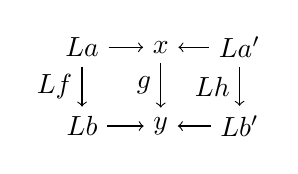
\begin{tikzpicture}
    % \draw [help lines, step=0.2, color=blue!10] (-5,-5) grid (5,5); % grid
    % % % % 
    \node (La) at (-1,1) {$ La $};
    \node (x) at (0,1) {$ x $};
    \node (La') at (1,1) {$ La' $};
    \node (Lb) at (-1,0) {$ Lb $};
    \node (y) at (0,0) {$ y $};
    \node (Lb') at (1,0) {$ Lb' $};
    \draw [->] (La) to node [] {$  $} (x);
    \draw [->] (La') to node [] {$  $} (x);
    \draw [->] (Lb) to node [] {$  $} (y);
    \draw [->] (Lb') to node [] {$  $} (y);
    \draw [->] (La) to node [left] {$ Lf $} (Lb);
    \draw [->] (x) to node [left] {$ g $} (y);
    \draw [->] (La') to node [left] {$ Lh $} (Lb');
  \end{tikzpicture}
\]
%%%%%%%%%%%%%%%%% 
%%%%%%%%%%%%%%%%% 
\end{document}
